\documentclass[a4paper]{article}

%------------------------------------------------------------
\usepackage[a4paper, total={6in, 9in}]{geometry}
\usepackage{algorithm}
\usepackage[noend]{algpseudocode}
\usepackage{amsmath}
\usepackage{booktabs}
\usepackage{caption}
\usepackage{enumitem}
\usepackage{graphicx}
\usepackage{float}
\usepackage{inconsolata}
\usepackage{listings}
\usepackage{pstricks-add}
\usepackage{siunitx}
\usepackage[most]{tcolorbox}
\usepackage{tikz}
\usepackage{epstopdf} %converting to PDF
\usepackage{hyperref}
\usepackage{rotating}

\usetikzlibrary{shapes.geometric}
\usetikzlibrary{calc}

%------------------------------------------------------------
\graphicspath{{./fig/}}

%------------------------------------------------------------
\setlength{\parindent}{0in}

\lstdefinestyle{Python}{
	language        = Python,
	basicstyle      = \ttfamily,
	keywordstyle    = \color{blue},
	keywordstyle    = [2] \color{teal}, % just to check that it works
	stringstyle     = \color{green},
	commentstyle    = \color{red}\ttfamily
}

%------------------------------------------------------------
\newtcblisting[auto counter]{sexylisting}[2][]{sharp corners, 
    fonttitle=\bfseries, colframe=gray, listing only, 
    listing options={basicstyle=\ttfamily,language=Python}, 
    title=Listing \thetcbcounter: #2, #1}

%------------------------------------------------------------
\tikzstyle{block} = [draw, fill=blue!20, rectangle, 
    minimum height=3em, minimum width=3em]
\tikzstyle{sum} = [draw, fill=blue!20, circle, node distance=1cm]
\tikzstyle{input} = [coordinate]
\tikzstyle{output} = [coordinate]
\tikzstyle{pinstyle} = [pin edge={to-,thin,black}]

%------------------------------------------------------------

\begin{document}
\title{SLAM: Map My World}
\author{Shane Reynolds}
\maketitle

\section*{Abstract}

\section{Introduction}
Consider a robot in an unknown environment, with no known map. The robot takes sensor readings and experiences control actions. Based on these observations and actions, the robot must construct a map and localise itself within the map. In robotics, this scenario is known as the \textit{simultaneous localisation and mapping problem}, or SLAM. In simpler terms, using sensor readings and control data, SLAM concurrently constructs an environment map, and determines the robots location and orientation within that map. This is an important problem since odometric data is subject to small perturbations which are introduced from wheel slippage and sensor noise - often refered to as odometric drift. Mapping allows a robot to revisit previously mapped terrain and reset any localisation error. Also, location and orientation within a given map are normally used as inputs for higher order functions like path planning. The problem is more difficult to solve than localisation with known poses since high dimensionality of map spaces can often lead to computational intractabilityy. This paper explores two approaches to solving SLAM. The first of these solutions is called FastSLAM which employs a combination of Extended Kalman Filters(EKF) and Monte Carlo Localisation (MCL) to solve the problem. The second approach is called GraphSLAM, which solves the problem by optimising a graph structure built by the algorithm. The paper concludes with an application of GraphSLAM in a Gazebo simulation using an off-the-shelf implementation called RTAB-Map in ROS. The GraphSLAM implementation is tested across two different environments providing opportunities for discussion of the algorithm robustness.

\section{Background}
Robot localisation aims to determine, for some discrete time step $t$, a distribution of the robot's pose, $x_t$, given a series of observations, $z_{1:t}$, control actions, $u_{1:t}$, and a map, $m$. The localisation problem is often expressed, using conditional probability notation, as follows:
\begin{equation}
p(x_t | z_{1:t}, m, u_{1:t})
\end{equation}

Mapping of an environment is the problem of determining a distribution over all possible map configurations, $m$, given a series of observations, $z_{1:t}$, and known robot poses, $x_{1:t}$. The mapping problem is often expressed, using conditional probability notation, as follows:
\begin{equation}
p(m | z_{1:t}, x_{1:t})
\end{equation}

Generally, a robot has neither the map, nor known poses, meaning that posteriors for both the map space and the robot's pose need to be determined. Equations (1) and (2) show these distributions are dependent on each other - evaluation of pose posterior requires the map, and evaluation of map posterior requires pose. This is often referred to as the chicken and egg problem. The main implication is that approaches designed to solve equations (1) and (2) cannot be readily applied in their current forms. Further, the problem can no longer be sufficiently expressed using these equations. SLAM, as the name suggests, determines these the map, $m$, and pose, $x_t$, simultaneously given sensor observations, $z_{1:t}$, and control actions, $u_{1:t}$. Mathematically, this is expressed as:
\begin{equation}
p(x_t, m | z_{1:t}, u_{1:t})
\end{equation}

Equation (3) is the equation for the \textit{online} SLAM problem, which is only concerned with determining the robot's current location. Another variation of the SLAM problem, which is more difficult to solve, is the \textit{full} SLAM problem. The \textit{full} SLAM problem seeks to determine the complete pose history of the robot, $x_{1:t}$. This is often expressed as follows:
\begin{equation}
p(x_{1:t}, m | z_{1:t}, u_{1:t})
\end{equation}

Typically, \textit{online} SLAM is used to dynamically localise the robot, whilst \textit{full} SLAM is determine offline and is used to determine where the robot has been. It is not hard to see that the solution to the \textit{online} SLAM problem can be determined by solving the \textit{full} SLAM problem and integrating - the relationship between the two problems can be seen in equation (XXXX):
\begin{equation}
p(x_t, m | z_{1:t}, u_{1:t}) = \int_{x_{t-1}} \int_{x_{t-2}} \dots \int_{x_1} p(x_{1:t}, m | z_{1:t}, u_{1:t}) dx_1 dx_2 \dots dx_{t-1}
\end{equation}

One final aspect of the SLAM problem has to do with determining whether or not the robot has previously encountered a feature in the map. The recognition of a map feature is discretely modelled: either the robot has encountered the feature before, or it has not. The literature refers to these recognitions as \textit{correspondences}, and correspendence $i$ is denoted as $c_i$. Rewriting the \textit{online} SLAM problem shown in equation (3) yields:
\begin{equation}
p(x_t, m, c_t \ | \ z_{1:t}, u_{1:t})
\end{equation}

Similarly, rewriting the \textit{full} SLAM problem shown in equation (4) yields:
\begin{equation}
p(x_{1:t}, m, c_{1:t} \ | \ z_{1:t}, u_{1:t})
\end{equation}

Finally, the \textit{online} and \textit{full} SLAM problems, with correspondences, can be linked similarly to equation (XXXX):
\begin{equation}
p(x_t, m, c_t | z_{1:t}, u_{1:t}) = \int_{x_{t-1}} \int_{x_{t-2}} \dots \int_{x_1} \sum_{c_1} \sum_{c_2} \dots \sum_{c_{t-1}} p(x_{1:t}, m | z_{1:t}, u_{1:t}) dx_1 dx_2 \dots dx_{t-1}
\end{equation}

This paper discusses two approaches for solving the SLAM problem. The first method is Grid Based Fast SLAM, introduced in subsection 2.1; the second method is Graph SLAM introduced in subsection 2.2.

\subsection{Grid Based FastSLAM}
FastSLAM was first proposed by XXXX. The central idea was an application of Rao-Blackwellized particle filter to estimate the joint posterior (reference to Murphy). To reduce the state space dimensionality, and hence the problem complexity, we will consider the problem with known correspondences, hence the joint posterior we are solving for is the one shown in equation (4). Using the simple Bayes' rule, $p(x_1,x_2) = p(x_2|x_1) \cdot p(x_1)$, equation (4) can be re-expressed as follows:
\begin{equation}
p(x_{1:t}, m | z_{1:t}, u_{1:t}) = p(x_{1:t} | z_{1:t}, u_{1:t}) \cdot p(m | x_{1:t}, z_{1:t}, u_{1:t})
\end{equation}

The key assumption made in Murphy's paper was that if the robot's path, $x_{1:t}$, is known then landmark locations are conditionally independent given the poses. This assumption allows us to factorise equation (5) as follows:
\begin{equation}
p(x_{1:t}, m | z_{1:t}, u_{1:t}) = p(x_{1:t} | z_{1:t}, u_{1:t}) \cdot \prod_{i} p(m_i | x_{1:t}, z_{1:t}, u_{1:t})
\end{equation}

Applying Bayes' theorem and then factorisation breaks the problem into two smaller problems: estimation of the robot path $p(x_{1:t} | z_{1:t}, u_{1:t})$; and estimation of the robot map $\prod_{i}p(m_i | x_{1:t}, z_{1:t}, u_{1:t})$. These smaller problems are known as the \textit{localisation} problem, and \textit{mapping} problem, respectively. Considering the problem in this light hints at an iterative approach to solving SLAM which consists of two steps: calculate the robot position; and then update the map based on that position. Grid based FastSLAM uses a particle filter to solve the localisation problem, such as Monte Carlo Localisation (MCL). The mapping problem is addressed using the \textit{occupancy grid mapping} algorithm, discussed in XXXX. The full Grid Based Fast SLAM algorithm can be seen in section 2.1.2.


\subsubsection{Occupancy Grid Mapping}
A common technique for map representation is to decompose a continuous environment, $m$, into a discrete grid representation such that:
\begin{equation}
m = \sum_{i} m_i
\end{equation}

Each cell, $m_i$, is either occupied or unoccupied. This representation, first introduced by XXXX, is referred to as an occupancy grid map.
\begin{figure}[h]
\centering
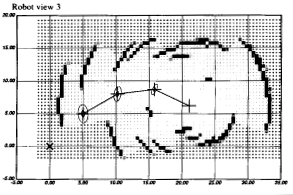
\includegraphics[scale=0.8]{occupancy_grid}
\caption{text}
\end{figure}

As previously mentioned, the mapping problem requires estimation of the posterior $p(m | x_{1:t}, z_{1:t})$. The main problem with estimating this posterior using a discrete grid cell representation is the high dimensionality. An example of this can be seen  by considering a map broken down into 500 discrete cells. If each cell is either occupied or unoccupied, then the total number of different maps that exist are $2^{500}$. Estimating $p(m | x_{1:t}, z_{1:t})$ requires determining the probability for each of the $2^{500}$ maps. This is computationally intractable for a system which needs to operate in real time. Instead of attempting this, occupancy grid algorithms estimate $p(m_i | x_{1:t}, z_{1:t})$ for each grid cell $m_i$. Considering the occupancy of each grid cell as independent from other grid cells, whilst not strictly true, is a convenient assumption allowing the expression expression of the posterior $p(m | x_{1:t}, z_{1:t})$ as a product of it's marginals:
\begin{equation}
p(m | x_{1:t}, z_{1:t}) = \prod_{i} p(m_i | x_{1:t}, z_{1:t})
\end{equation}

We note that $p(m_i | x_{1:t}, z_{1:t})$ in equation (XXXX) is estimating a fixed binary quantity from a sequence of sensor measurements. According to XXXX beliefs of this type are commonly implemented as \textit{log odds ratios}. We note that the \textit{odds} of a state is defined as the ratio of the probability of the binary event divided by the probability of its negate. Using Bayes' theorem, we express $p(m_i | x_{1:t}, z_{1:t})$ as follows:
\begin{equation}
p(m_i | x_{1:t}, z_{1:t}) = \frac{p(z_t | m_i, z_{1:t-1}, x_{1:t}) \cdot p(m_i | z_{1:t}, x_{1:t})}{p(z_t | z_{1:t-1}, x_{1:t})}
\end{equation}

Applying the Markov assumption for the first term in the numerator yields:
\begin{equation}
p(m_i | x_{1:t}, z_{1:t}) = \frac{p(z_t | m_i, x_{t}) \cdot p(m_i | z_{1:t}, x_{1:t})}{p(z_t | z_{1:t-1}, x_{1:t})}
\end{equation}

We note, applying Bayes' theorem, that:
\begin{equation}
p(z_t | m_i, x_t) = \frac{p(m_i | z_t, x_t) \cdot p(z_t | x_t)}{p(m_i | x_t)}
\end{equation}

Using equation (XXXX), we can re-express equation (XXXX) as:
\begin{equation}
p(m_i | x_{1:t}, z_{1:t}) = \frac{p(m_i | z_t, x_t) \cdot p(z_t | x_t) \cdot p(m_i | z_{1:t-1}, x_{1:t-1})}{p(m_i | x_t) \cdot p(z_t | z_{1:t-1}, x_{1:t})}
\end{equation}

A further application of the Markov assumption allows us to express equation (XXXX) as:
\begin{equation}
p(m_i | x_{1:t}, z_{1:t}) = \frac{p(m_i | z_t, x_t) \cdot p(z_t | x_t) \cdot p(m_i | z_{1:t-1}, x_{1:t-1})}{p(m_i) \cdot p(z_t | z_{1:t-1}, x_{1:t})}
\end{equation}

Similarly, we can follow the same process for the negate of $m_i$, $\neg m_i$. This yields the following expression:
\begin{equation}
p(\neg m_i | x_{1:t}, z_{1:t}) = \frac{p(\neg m_i | z_t, x_t) \cdot p(z_t | x_t) \cdot p(\neg m_i | z_{1:t-1}, x_{1:t-1})}{p( \neg m_i) \cdot p(z_t | z_{1:t-1}, x_{1:t})}
\end{equation}

Hence, after some manipulation, the \textit{odds} can be expressed as:
\begin{equation}
\frac{p(m_i | z_{1:t}, u_{1:t})}{p( \neg m_i | z_{1:t}, u_{1:t})} = \frac{p(m_i | z_t, x_t)}{1 - p(m_i | z_t, x_t)} \cdot \frac{p(m_i | z_{1:t-1}, x_{1:t-1})}{1 - p(m_i | z_{1:t-1}, x_{1:t-1})} \cdot \frac{1 - p(m_i)}{p(m_i)}
\end{equation}

Taking the logarithm of this yields the the \textit{log odds} calculation, $l_t$, for single grid cell:
\begin{equation}
l_t = \log \bigg( \frac{p(m_i | z_t, x_t)}{1 - p(m_i | z_t, x_t)} \bigg) + \log \bigg( \frac{p(m_i | z_{1:t-1}, x_{1:t-1})}{1 - p(m_i | z_{1:t-1}, x_{1:t-1})} \bigg) + \log \bigg( \frac{1 - p(m_i)}{p(m_i)} \bigg)
\end{equation}

We note that equation (XXXX) can be expressed recursively since the middle term is just $l_{t-1}$. Further, the inverted final term is simply the inital belief $l_0$ Hence, we get:
\begin{equation}
l_t = l_{t-1} + \log \bigg( \frac{p(m_i | z_t, x_t)}{1 - p(m_i | z_t, x_t)} \bigg) - l_0
\end{equation}

The final term in equation (XXXX) is just the initial belief for the grid cell, and the second to last term is referred to as the \textit{inverse sensor model}. The occupancy grid mapping algorithm takes the current pose $x_t$ and current sensor measurements $z_t$, along with the array of log odds ratios calculated in a previous iteration for each grid cell. This array is denoted as $\{l_{t-1,i}\}$. The algorithm simply loops through all of the grid cells which comprise an environmental map, updating the log odds ratio for each cell. The pseudo code for the occupancy grid algorithm can be seen below.

\begin{algorithm}[h]
\caption{Occupancy Grid Mapping}
\begin{algorithmic}[1]
\Procedure{$\text{occupancy\_grid\_mapping}$}{$\{ l_{t-1,i} \}$, $x_t$, $z_t$}
\For{all cells $m_i$}
	\If{$m_i$ in preceptual field of $z_t$}
		\State $l_{t,i} = l_{t-1,i} + \text{inverse\_sensor\_model}(m_i, x_t, z_t) - l_0$
	\Else
		\State $l_{t,i} = l_{t-1,i}$
	\EndIf
\EndFor
\Return $\{ l_{t,i} \}$
\EndProcedure
\end{algorithmic}
\end{algorithm}

\newpage

\subsubsection{Grid Based FastSLAM Algorithm}
The grid based FastSLAM algorithm takes as input variable $X_{t-1}$, which holds the particles from a previous call to the algorithm. Each particle in $X_{t-1}$ consists of a hypothesised robot pose and map. Additionally, odometry $u_t$, and sensor measurements $z_t$ are also received as inputs. The algorithm commences by initialising empty variable $\hat{X}_t$ to store newly formed particle hypotheses. MCL is used to update the particle odometry from $X_{t-1}$, forming new pose hypotheses for each particle. Sensor measurements are used to determine the likelihood for each pose hypothesis. Using the updated pose hypotheses, the occupancy grid mapping algorithm is called, forming a map hypothesis for each particle. Once all of the existing particles from $X_{t-1}$ have been updated, then a re-sampling procedure commences, which sees particles selected at random according to their likelihood of existing calculated earlier. The final set of re-sampled particles is returned and the algorithm is completed. These set of particles form the new aggregate hypothesis of the robot's map, and pose within the map - over many iterations of the algorithm, the hypothesis will converge on the true map and robot pose. The full Grid Based FastSLAM algorithm can be seen in Algorithm 2 below.

\begin{algorithm}[h]
\caption{Grid Based FastSLAM}
\begin{algorithmic}[1]
\Procedure{$\text{gridbased\_fast\_slam}$}{$X_{t-1}$, $u_t$, $z_t$}
\State $\hat{X}_t = X_t = \emptyset$
\For{$k=1$ to $M$}
	\State $x_t^{[k]} = \text{sample\_motion\_model}(u_t, x_{t-1}^{[k-1]})$
	\State $\omega_t^{[k]} = \text{measurement\_model\_map}(z_t, x_t^{[k]}, m_{t-1}^{[k]})$
	\State $m_t^{[k]} = \text{updated\_occupancy\_grid}(z_t, x_t^{[k]}, m_{t-1}^{[k]})$
	\State $\hat{X}_t = \hat{X}_t \ \cup <x_t^{[k]}, m_t^{[k]}, \omega_t^{[k]}>$
\EndFor
\For{$k=1$ to $M$}
	\State draw $i$ from $\hat{X}_t$ with probability $\propto \omega_t^{[i]}$
	\State $X_t = X_t \ \cup <x_t^{[i]}, m_t^{[i]}>$
\EndFor
\Return $X_t$
\EndProcedure
\end{algorithmic}
\end{algorithm}

\subsection{GraphSLAM}
GraphSLAM, in comparison to GBFS, takes a fundamentally different approach to solving the SLAM problem. The main idea behind GraphSLAM is to build up a graph with nodes derived from robot poses, $x_t$, and map features, $m_t$. The graph edges represent a series of constraints. The constraints are used to develop a likelihood cost function - minimising this cost function is analogous to determining pose and map features that maximise the likelihood of measurement observations. Optimisation is achieved using classical optimisation techniques, and is performed off-line once the graph has been constructed. Often is its helpful to think of GraphSLAM as having a front end and a back end, as shown in Figure XXXX. The front end, which receives raw sensor data as input, focuses on graph construction. The back end receives the constructed graph as input, optimises the graph, and outputs map and trajectory estimation.
\begin{figure}[h]
\centering
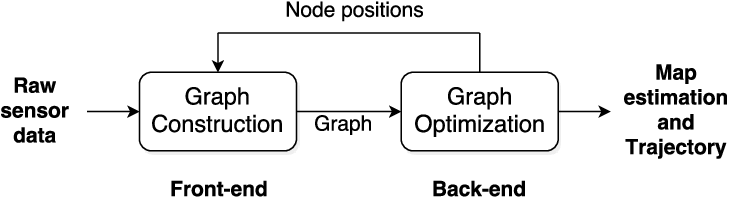
\includegraphics[scale=0.35]{Graph-SLAM-system}
\caption{text}
\end{figure}


\subsubsection{GraphSLAM Front End}
The front end of GraphSLAM is concerned with constructing the graph and determining the constraints. A robot nagivating some 2D topology typically has a pose comprised of position coordinates $x$, and $y$, as well as orientation $\theta$. To make things simple, we will encapsulate these three parameters in a single pose vector $x_t = \begin{bmatrix} x & y & \theta \end{bmatrix}$. To simplify things further often a single parameter is used to represent state variables that contain one or more poses $x_{0:t}$ with the map $m$. Thrun and Montemerlo define $y_{0:t}$ to be a vector composed of the path $x_{0:t}$ and the map $m$, whereas $y_t$ is simply composed as a single momentary pose in time, $x_t$, and the map $m$:
\begin{equation}
y_{0:t} =
\begin{bmatrix}
x_0 \\ x_1 \\ \vdots \\ x_t \\ m
\end{bmatrix}
\quad\mathrm{and}\quad 
y_t =
\begin{bmatrix}
x_t \\ m
\end{bmatrix}
\end{equation}

As the robot moves around the environment, it experiences control actions $u_{1:t}$, takes sensor measurements $z_{1:t}$, and develops correspondences $c_{1:t}$. The posterior of full SLAM seen in equation (4) can be expressed using $y_{0:t}$, which yields the following:
\begin{equation}
p(y_{0:t} \ | \ z_{1:t}, u_{1:t}, c_{1:t})
\end{equation}

Factorising equation XXXX using Bayes rule yields the following expression:
\begin{equation}
p(y_{0:t} \ | \ z_{1:t}, u_{1:t}, c_{1:t}) = \frac{p(z_t \ | \ y_{0:t}, z_{1:t-1}, u_{1:t}, c_{1:t}) \ p(y_{0:t} \ | \ z_{1:t-1}, u_{1:t}, c_{1:t})}{p(z_t \ | \ z_{1:t-1}, u_{1:t}, c_{1:t})}
\end{equation}

Letting $\eta = p(z_t \ | \ z_{1:t-1}, u_{1:t}, c_{1:t})^{-1}$, we simplify equation (XXXX) as follows:
\begin{equation}
p(y_{0:t} \ | \ z_{1:t}, u_{1:t}, c_{1:t}) = \eta \ p(z_t \ | \ y_{0:t}, z_{1:t-1}, u_{1:t}, c_{1:t}) \ p(y_{0:t} \ | \ z_{1:t-1}, u_{1:t}, c_{1:t})
\end{equation}

The \textit{Markov assumption} allows the simplification of the first probability in equation (XXXX):
\begin{equation}
p(y_{0:t} \ | \ z_{1:t}, u_{1:t}, c_{1:t}) = \eta \ p(z_t \ | \ y_t, c_t) \ p(y_{0:t} \ | \ z_{1:t-1}, u_{1:t}, c_{1:t})
\end{equation}

Partitioning $y_{0:t}$ into $x_t$ and $y_{0:t-1}$ the second probability term in equation (XXXX) can be expressed as:
\begin{equation}
p(y_{0:t} \ | \ z_{1:t-1}, u_{1:t}, c_{1:t}) = p(x_t \ | \ y_{0:t-1}, z_{1:t-1}, u_{1:t}, c_{1:t}) \ p(y_{0:t-1} \ | \ z_{1:t-1}, u_{1:t}, c_{1:t})
\end{equation}
\\
THERE IS AN ADDITIONAL STEP HERE
\\

Substituting equation (XXXX) back into equation (XXXX) yields a recursive expression for the full SLAM posterior:
\begin{equation}
p(y_{0:t} \ | \ z_{1:t}, u_{1:t}, c_{1:t}) = \eta \ p(z_t \ | \ y_t, c_t) \ p(x_t \ | \ x_{t-1}, u_t) \ p(y_{0:t-1} \ | \ z_{1:t-1}, u_{1:t-1}, c_{1:t-1})
\end{equation}

Mathematical induction over $t$ yields the closed form solution where $p(y_0)$ is the prior over the map $m$ and the initial pose $x_0$. The closed form solution is:
\begin{equation}
p(y_{0:t} \ | \ z_{1:t}, u_{1:t}, c_{1:t}) = \eta \ p(y_0) \ \prod_{t} p(x_t \ | \ x_{t-1}, u_t) p(z_t \ | \ y_t, c_t)
\end{equation}

We note that probability $p(x_t \ | \ x_{t-1}, u_t)$ is the \textit{motion model}, which gives us the probability of our current pose, $x_t$, given the previous pose and our odometry $u_t$. The other probability, $p(z_t \ | \ y_t, c_t)$, is the \textit{sensor model} - this gives us the probability of receiving the sensor measurements given the current position, map, and correspondences. Equation (XXXX) is important because it allows us to think of the full SLAM posterior as a series of independent probabilistic events. Our task now becomes one of optimisation: how should we select $x_{0:t}$ and $m$ so that we maximise the probability $p(y_{0:t} \ | \ z_{1:t}, u_{1:t}, c_{1:t})$. Maximising a set of additive terms is much easier than maximising a set of multiplicative terms, and so we take a log transform which gives us:
\begin{equation}
\log p(y_{0:t} \ | \ z_{1:t}, u_{1:t}, c_{1:t}) = \log \eta + \log p(y_0) + \sum_{t} \bigg[ \log p(x_t | x_{t-1}, u_t)  \bigg] + \sum_{t} \bigg[ \log p(z_t | y_t, c_t)  \bigg]
\end{equation}

We assume that the robot motion is distributed normally according to $\mathcal{N}(g(u_t, x_{t-1}), R_t)$, where $g$ is the deterministic motion function, and $R_t$ is the covariance of the motion error. Similarly, measurements $z_t$ are generated according to $\mathcal{N}(h(y_t, c_t), Q_t)$, where $h$ is the measurement function and $Q_t$ is the measurement error covariance. Multivariate normal pdf, where $K_1$ is used to represent the leading scalar coefficient, allows us to express the \textit{motion model} as:
\begin{equation}
p(x_t|x_{t-1}, u_t) = K_1 \exp \bigg\{ -\frac{1}{2}(x_t - g(u_t, x_{t-1}))^T R_t^{-1} (x_t - g(u_t, x_{t-1})) \bigg\}
\end{equation}

Similarly, we can express the \textit{sensor model} as:
\begin{equation}
p(z_t|y_t, c_t) = K_2 \exp \bigg\{ -\frac{1}{2}(z_t - h(y_t,c_t))^T Q_t^{-1} (z_t - h(y_t,c_t)) \bigg\}
\end{equation}

Noting that the prior $p(y_0)$ can be factorised into two independent priors $p(x_0)$ and $p(m)$, we typically just replace $p(y_0)$ with $p(x_0)$ since we often have no prior knowledge about the map - $p(m)$ is often subsumed by the normaliser $\eta$. With this in mind, we also express the prior $p(x_0)$ with a Gaussian type distribution:
\begin{equation}
p(x_0) = K_3 \exp \bigg\{ -\frac{1}{2} x_0^T \Omega_0 x_0 \bigg\}
\end{equation}

with
\begin{equation}
\Omega_0 =
\begin{bmatrix}
\infty & 0      & 0 \\
0 	   & \infty & 0 \\
0 	   & 0 		& \infty
\end{bmatrix}
\end{equation}

Substituting equations (XX), (XX), and (XX) into equation (XX) and putting constants $\log \eta$, $\log K_1$, $\log K_2$, and $\log K_3$ into $C$, we can express the negative of equation (XX) as:
\begin{align}
-\log p(y_{0:t}|z_{1:t}, u_{1:t}, c_{1:t}) = C &+ \frac{1}{2} \cdot x_0^T \Omega_0 x_0 \nonumber \\ &+ \frac{1}{2} \cdot \sum_{t} (x_t - g(u_t, x_{t-1}))^T R_t^{-1} (x_t - g(u_t, x_{t-1})) \nonumber \\ &+ \frac{1}{2} \cdot \sum_{t} (z_t - h(y_t,c_t))^T Q_t^{-1} (z_t - h(y_t,c_t))
\end{align}

Determining the robot trajectory and map by minimising equation (XX) is the same as maximising equation (XX). In the literature, equation (XX) often has the scalar coefficients removed and is referred to as $J_{GraphSLAM}$. This is expressed as:
\begin{align}
J_{GraphSLAM} = C &+ x_0^T \Omega_0 x_0 \nonumber \\ &+ \sum_{t} (x_t - g(u_t, x_{t-1}))^T R_t^{-1} (x_t - g(u_t, x_{t-1})) \nonumber \\ &+ \sum_{t} (z_t - h(y_t,c_t))^T Q_t^{-1} (z_t - h(y_t,c_t))
\end{align}

Another important way to think about equation (XX) is as the sum of constraints derived from the edges of a graph. As the robot moves around the environment, it forms pose nodes periodically. Additionally, it forms map feature nodes from sensor measurements. Edges between two corresponding pose nodes are referred to as motion constraints, and are derived from odometry sensor data - these are represented using notation $u_t$. Edges between poses and map features are referred to as measurement constraints, and are derived from exteroceptive sensors - these are represented using notation $z_t$. An example of a graph composed of pose nodes and map feature nodes can be seen in Figure XXXX. The robot moves from pose $x_0$ to pose $x_1$, and so on. As the robot moves, sensors detect map features $m_1$ and $m_2$. Odometric measurements are captured and used to create edges $u_0$, $u_1$, and $u_2$. Additionally, exteroceptive sensors capture the distance from the robot location to the map features resulting in dashed line edges $z_0$, $z_1$, $z_2$, and $z_3$.
\begin{figure}[h]
\centering
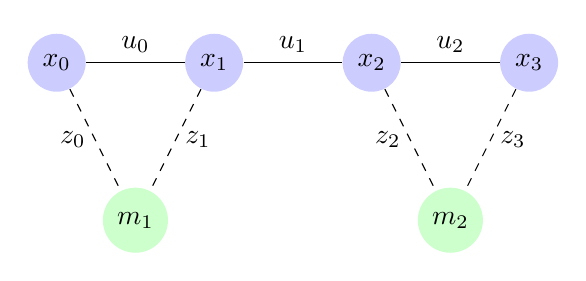
\begin{tikzpicture}
% Draw the nodes used for the picture
\node[circle,fill=blue!20](a){$x_0$};
\node[circle,fill=blue!20,right of=a,node distance=2cm](b){$x_1$};
\node[circle,fill=blue!20,right of=b,node distance=2cm](c){$x_2$};
\node[circle,fill=blue!20,right of=c,node distance=2cm](d){$x_3$};
\node(e) at ($(a)!0.5!(b)$){};
\node(f) at ($(c)!0.5!(d)$){};
\node[circle,fill=green!20,below of=e,node distance=2cm](g){$m_1$};
\node[circle,fill=green!20,below of=f,node distance=2cm](h){$m_2$};

% Draw the edges between the nodes
\draw (a) -- node[above]{$u_0$} (b);
\draw (b) -- node[above]{$u_1$} (c);
\draw (c) -- node[above]{$u_2$} (d);
\draw[dashed] (a) -- node[left]{$z_0$} (g);
\draw[dashed] (b) -- node[right]{$z_1$} (g);
\draw[dashed] (c) -- node[left]{$z_2$} (h);
\draw[dashed] (d) -- node[right]{$z_3$} (h);
\end{tikzpicture}
\caption{text}
\end{figure}

Once a set of constraints have been formed, $J_{GraphSLAM}$ can be found by simply summing the constraints together. Building a graph from pose and measurement nodes, and the subsequent constraint determination is the way that the front end of Graph SLAM is implemented. Once the graph has been determined, it is then passed to the back end for optimisation to determine the robot trajectory and map.

\subsubsection{GraphSlam Back End}
The back end of GraphSLAM is concerned with optimising the developed graph. There are a couple of ways to think about this if the constraints were all linear (or linearised) then we can find the maximum of the manifold surface by simply taking the derivative for each dimension and solve the resulting system of equations. The system is typically written as the following $\Omega \cdot \mu = \xi$. We note that $\Omega$ is referred to as the information matrix, and $\xi$ the information vector. Alternatively an optimisation algorithm such as Stochstic Gradient Descent 


\subsubsection{RTAB Map Impementation}
RTAB-Map is a graph-based SLAM approach that has been integrated in ROS. The \textit{rtabmap} node, seen in Figure XXXX, takes ROS \textit{tf} input to determine the position of the sensors in relation to the robot base; Odometry from any source such as rotary encoders or IMU; camera input from either RGB-D or stereo cameras; and an optional input from either 2D lidar, point cloud data from 3D lidar.
\begin{figure}[h]
\centering
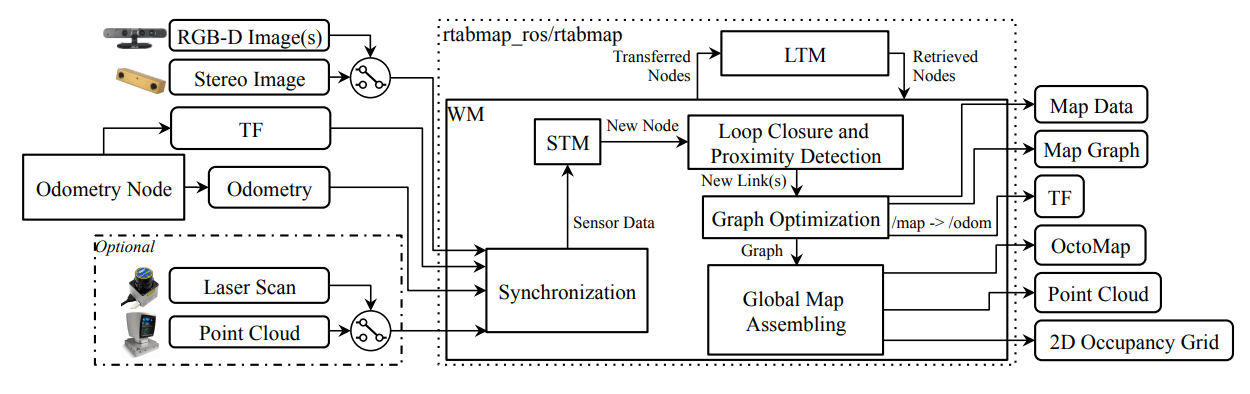
\includegraphics[scale=0.3]{rtabmap_node}
\caption{text}
\end{figure}

After sensor input has been synchronised, the Short-Term Memory (STM) module creates a node which remembers odometry pose, raw data from sensors, and additional information such as visual words for Loop Closure. Nodes are created every few millisecond at a predetermined frequency. As sequential nodes are created constraints are formed linking nodes together. Constraints come in three flavours: Neighbour, Loop Closure, and Proximity. Neighbour constraints are added in the STM between consecutive nodes with odometry transformation. Loop Closure and Proximity constraints are added through loop closure detection or proximity detection, respectively. Graph optimisation propagates computed error to the whole graph each time a new loop closure or proximity constraint is added to the graph - this helps to rectify odometry drift.


\section{Scene and robot configuration}
\subsection{Robot Model}
A robot model with simple geometries was selected for use in the SLAM simulation. The chassis is a rectangular prisim, and two wheels are located either side of the chassis centre forming a differential drive configuration - the robot model can be seein in Figure XXXX. An RGBD camera, front mounted on the chassis, provides 3D point cloud data of the environment and is represented by a red cube. Finally, a laser range finder is mounted on top of the robot providing 2D planar depth information.\\

\begin{figure}[h]
\begin{minipage}{0.45\textwidth}
	\centering
	\frame{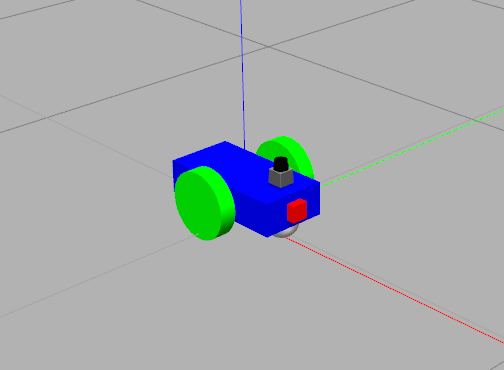
\includegraphics[scale=0.35]{robot_model}}
	\caption{text}
\end{minipage}
\hspace{1cm}
\begin{minipage}{0.45\textwidth}
	\captionof{table}{heading}
	\begin{tabular}{ll}
		\toprule
		\textbf{Link} & \textbf{Parent Link} \\
		\midrule
		\texttt{robot\_footprint} & \texttt{odom} \\
		\texttt{chassis} & \texttt{robot\_footprint} \\
		\texttt{camera} & \texttt{chassis} \\
		\texttt{hokuyo} & \texttt{chassis} \\
		\texttt{left\_wheel} & \texttt{chassis} \\
		\texttt{right\_wheel} & \texttt{chassis} \\
		\texttt{camera\_link\_optical} & \texttt{camera} \\
		\bottomrule
	\end{tabular}
\end{minipage}
\end{figure}

A full list of the links used to construct the robot model in the \texttt{graph\_slam\_bot.xacro} xml file can be seen in Table XXXX. Pictorially, the 3D coordinate frame hierachy is shown in Figure XXXX. This shows the coordinate frame attached to each link, in addition to the coordinate fram used for odometry. Note that arrows go from parent frames to child frames.

\clearpage

\begin{sidewaysfigure}[h]
	\centering
	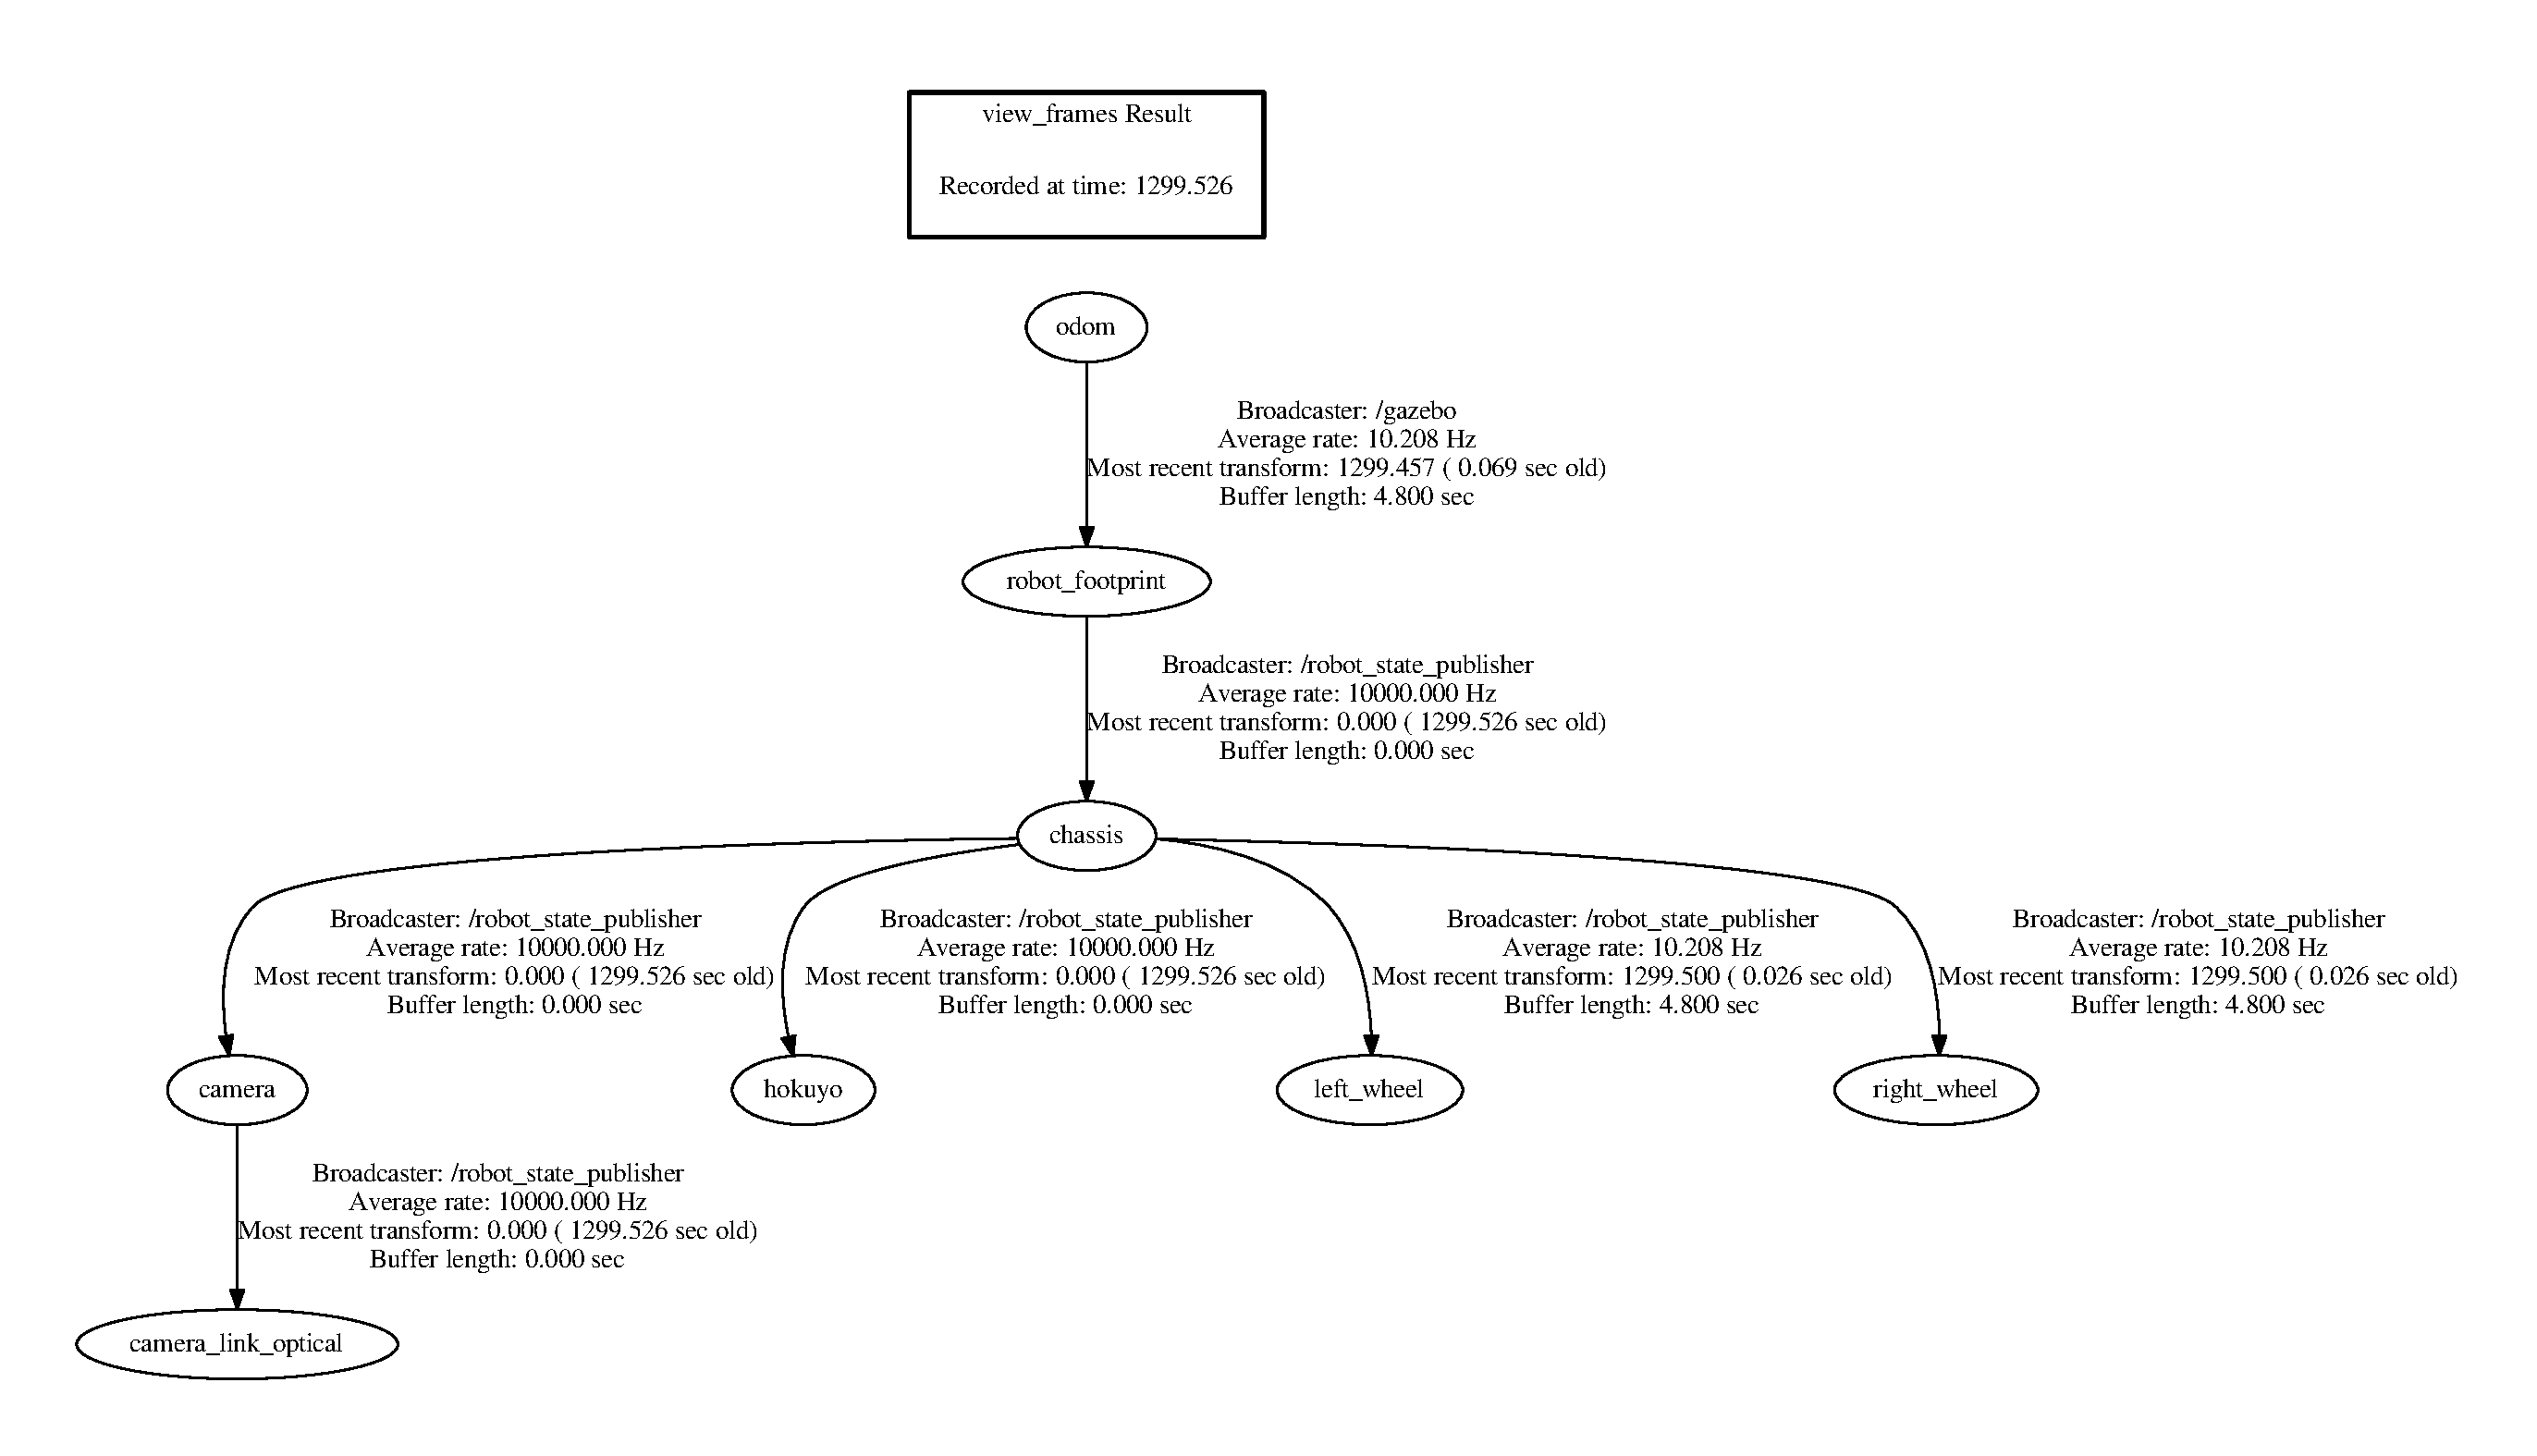
\includegraphics[scale=0.5]{frames}
	\caption{text}
\end{sidewaysfigure}

\clearpage

RTAB-Map is the package used to equip the robot model with GraphSLAM capabilities. The package uses RGB-D or stereo cameras and Lidar, meaning that there is some configuration of the RTAB-Map node to ensure that it is correctly subscribed to the correct topics published from the robot model sensors. A block diagram of the suggested configuration for robot models employing both RGB-D and Lidar can be seen in Figure XXXX. Notably, there are three topics for subsctiption from the RGB-D camera: RGB Image, Camera Info, and Image Depth. The Laser Scan and Odometry need to be subscribed from the published Lidar and rotary encoders topics, respectively.

\begin{figure}[h]
	\centering
	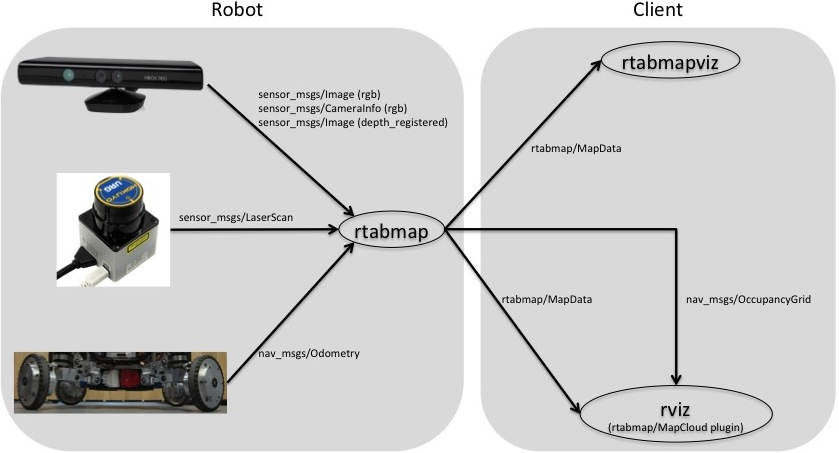
\includegraphics[scale=0.5]{rtabmap_setup}
	\caption{text}
\end{figure}

\begin{table}[h]
	\centering
	\caption{text}
	\begin{tabular}{ll}
		\toprule
		\textbf{Sensor Topic} & \textbf{Topic Path} \\
		\midrule
		RGBD Camera Image & \texttt{/camera\_ir/rgb/image\_raw} \\
		RGBD Camera Depth & \texttt{/camera\_ir/depth/image\_raw} \\
		RGBD Camera Info & \texttt{/camera\_ir/rgb/camera\_info} \\
		Laser Scan & \texttt{/graph\_slam\_bot/laser/scan} \\
		Odometry & \texttt{} \\ 
		\bottomrule
	\end{tabular}
\end{table}

\begin{figure}[h]
	\begin{minipage}{0.45\textwidth}
		text
	\end{minipage}
	\hspace{0.5cm}
	\begin{minipage}{0.45\textwidth}
		\centering
		\captionof{table}{text}
		\begin{tabular}{cc}
			\toprule
			\textbf{Parameter} & \textbf{Value}\\
			\midrule
			\texttt{Grid/FromDepth} & \texttt{false} \\
			\texttt{subscribe\_scan} & \texttt{true} \\
			\texttt{subscribe\_depth} & \texttt{true} \\
			\bottomrule
		\end{tabular}
	\end{minipage}
\end{figure}

\clearpage

\begin{sidewaysfigure}[h]
	\centering
	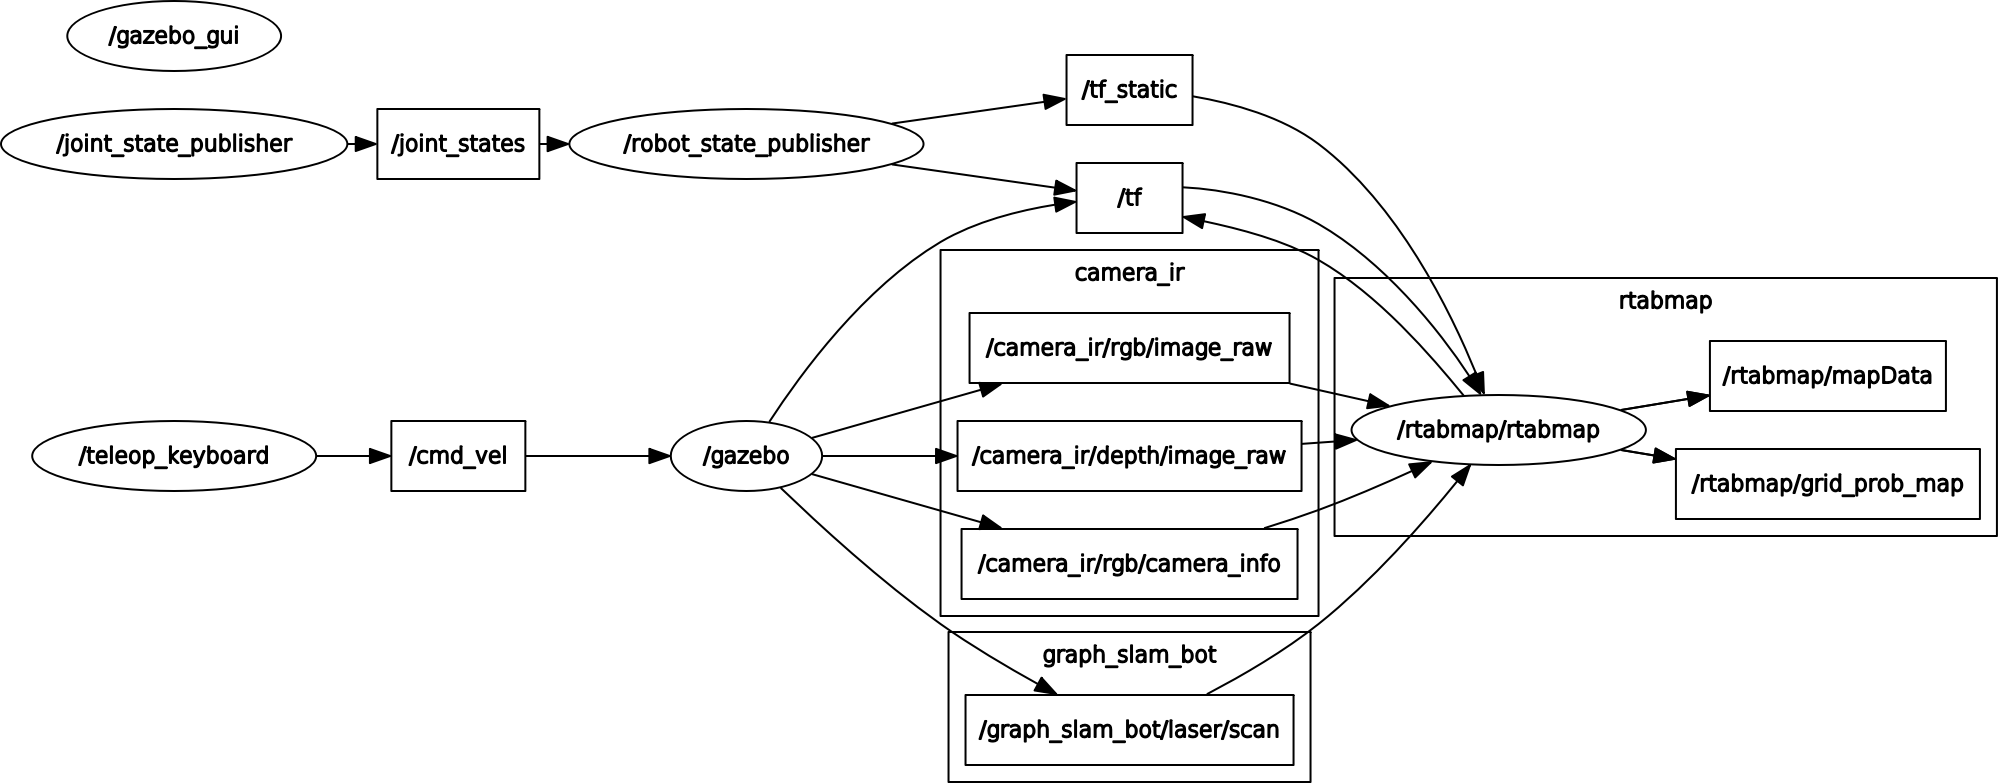
\includegraphics[scale=0.4]{rosgraph}
	\caption{text}
\end{sidewaysfigure}

\clearpage


WHAT ARE THE MAIN FILES THAT WERE REQUIRED TO CONFIGURE THE ROBOT

TALK ABOUT THE LAUNCH FILES THAT WERE CREATED TO LAUNCH EACH OF THE RESPECTIVE NODES


\subsection{Environment Model}
Rtab-Map was tested in two different environment models: a benchmark model, and an alternative model. Models have differing topologies, sizes, and features. 

\subsubsection{Benchmark Environment}
The benchmark model is of a small apartment mock up, featuring a kitchen and lounge room. The model is highly textured and contains many features - a good representation of real world environments. Rtab-Map should perform well in this environment because it is visually rich providing many opportunities for loop closure. The robot spawn point is in the kitchen. The benchmark environment model can be seen in Figure XXXX.

\begin{figure}[h]
\centering
\frame{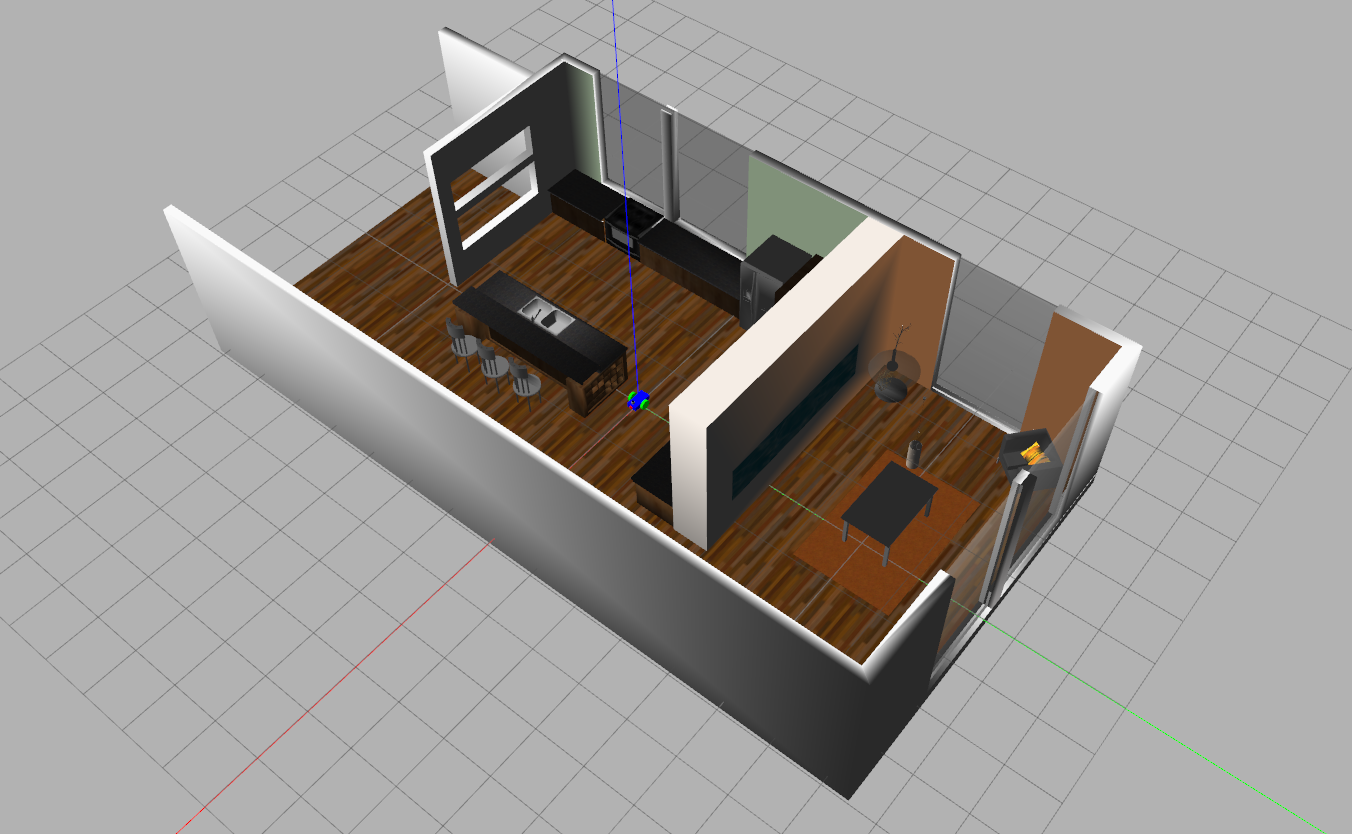
\includegraphics[scale=0.3]{benchmark_env}}
\caption{text}
\end{figure}

\subsubsection{Alternative Environment}
The alternative model was designed to be very simple. The topology is a basic rectangular room. An important design feature is the variation of features in the environment: some areas have many features, and other areas are featureless. This design choice was made to help evaluate Rtab-Map's performance in sections of the environment that are visually bland, or that have repetitive textures. The environment model was developed using the building editor embedded in Gazebo. The alternative environment model can be seen in Figure XXXX.

\begin{figure}[h]
\centering
\frame{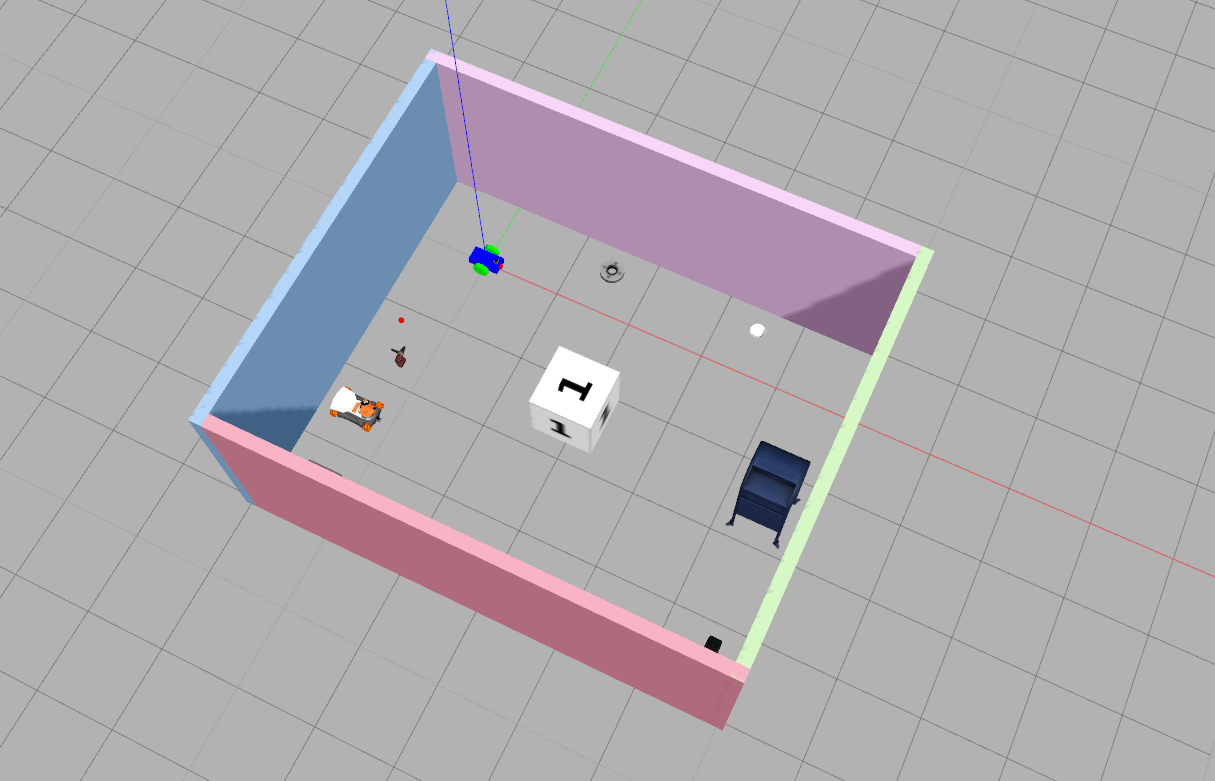
\includegraphics[scale=0.3]{alternative_env}}
\caption{text}
\end{figure}

\section{Results}
\subsection{Benchmark Environment}
A teleop node was set up to manoeuvre the robot around the benchmark environment using keyboard input control. Approximately three laps of the kitchen, balcony, and lounge room areas were performed. Figure XXXX shows a final iteration of the 2D occupancy grid map, in addition to blue line which represents the robot's node graph through the environment, which is optimised by GraphSLAM in Rtab-Map. The red lines connecting nodes show loop closure activity. The red and green coordinate axes show the robot's starting location.
\begin{figure}[h]
\centering
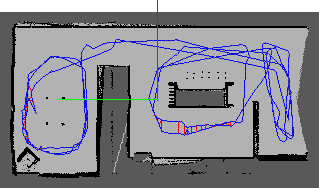
\includegraphics[scale=0.8]{kitchen_graph_view}
\caption{text}
\end{figure}

As the robot traverses the environment Rtab-Map identifies features from images using the \texttt{SURF} detection algorithm which was specified in the mapping node configuration. Figure XXXX shows a single image along the robot path, taken from the Rtab-Map database. The yellow highlights identify features that \texttt{SURF} has identified. As images are collected along the robot path, features in new images are compared to features from old images. The pink highlights represent instances where two images have features in common. These common features are used to create neighbouring links between images and loop closures. Figure XXXX shows the constraint view for the same point in time as Figure XXXX - this shows where the neighbouring links and loop closures were created.
\begin{figure}[h]
\centering
\begin{minipage}[t]{0.45\textwidth}
\centering
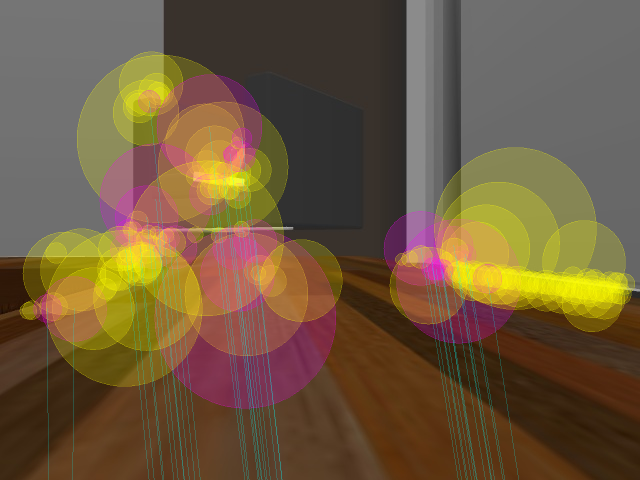
\includegraphics[height=5.5cm]{kitchen_features}
\caption{text}
\end{minipage}
\hspace{1cm}
\begin{minipage}[t]{0.45\textwidth}
\centering
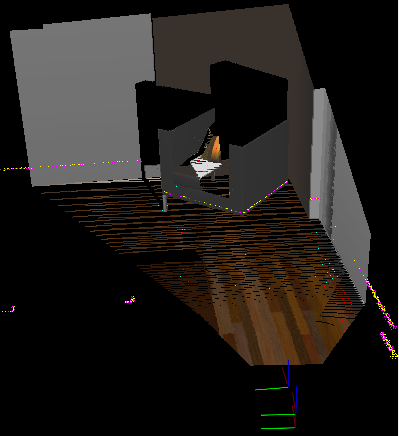
\includegraphics[height=5.5cm]{kitchen_constraints}
\caption{text}
\end{minipage}
\end{figure}

NEED TO TALK MORE ABOUT THE DIFFERENT LOOP CLOSURE ACTIVITY AND ACTIVITY WHERE THERE WAS NO LOOP CLOSURE.

Rtab-Map successfully created a 3D map from captured point cloud data captured by the RGBD camera. The 3D environment model was of reasonable fidelity, and well aligned with the 2D occupancy grid. Figure XXXX shows the 3D environment model from Rviz.
\begin{figure}[h]
\centering
\frame{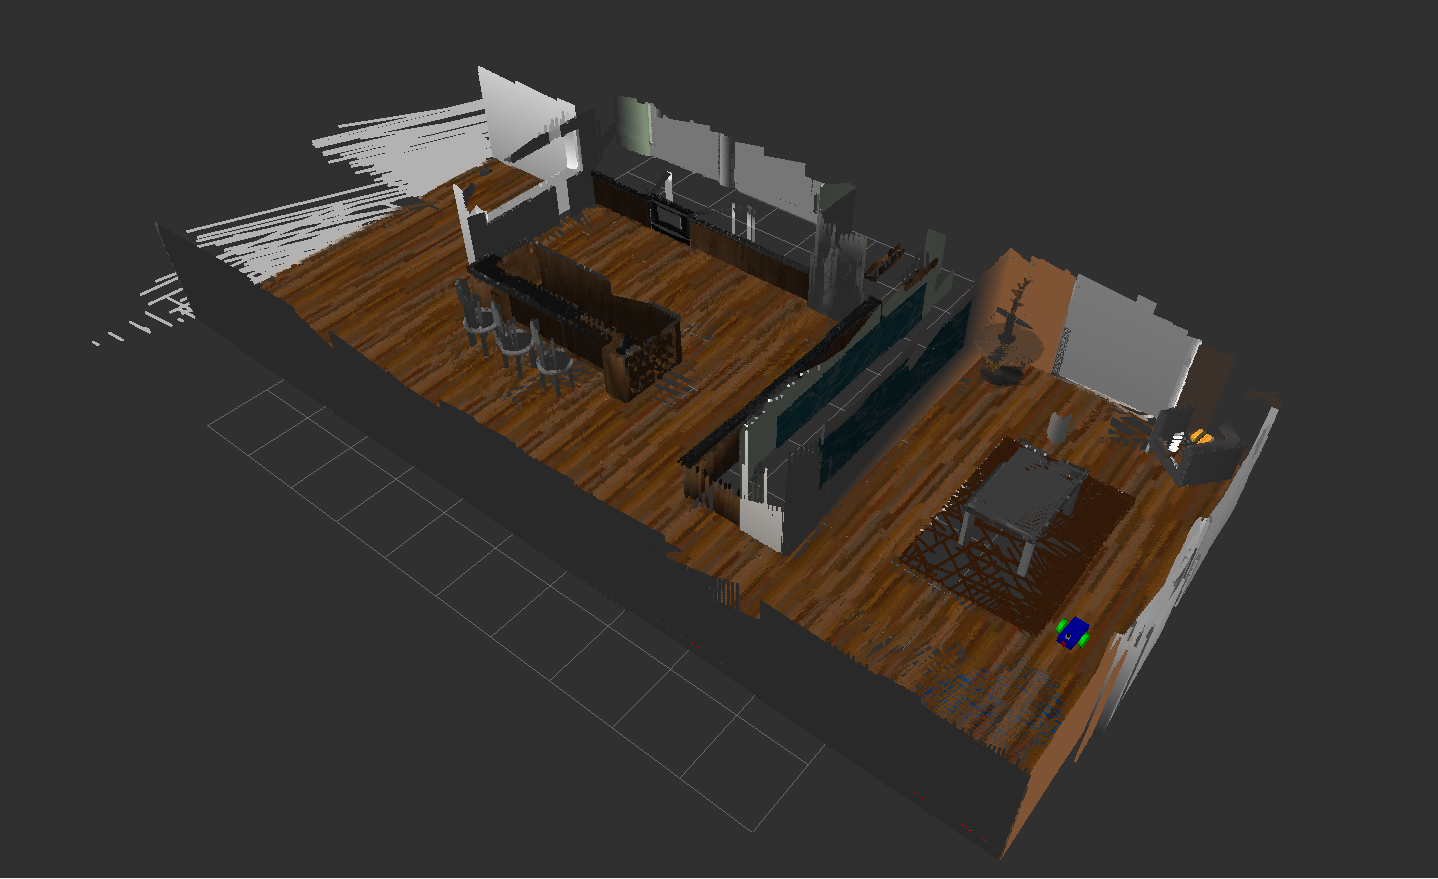
\includegraphics[scale=0.28]{kitchen_3d_map_2}}
\caption{text}
\end{figure}

The robot was able to successfully localise within the mapped environment, making small corrections to the odometry upon detection of loop closure.


\subsection{Alternative Environment}
As with the benchmark model, the robot was manoeuvred through the alternative environment using keyboard commands issued to a teleop node. Three laps of the basic environment were undertaken. The final iteration of the 2D occupancy grid map can be seen in Figure XXXX. The node graph used by GraphSLAM in Rtab-Map is represented by the blue line, and loop closure activity is shown in red.
\begin{figure}[h]
\centering
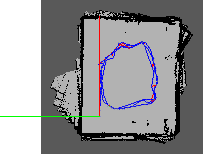
\includegraphics[scale=1.2]{slam_house_2_graph_view}
\caption{text}
\end{figure}

\begin{figure}[h]
\centering
\begin{minipage}{0.45\textwidth}
\centering
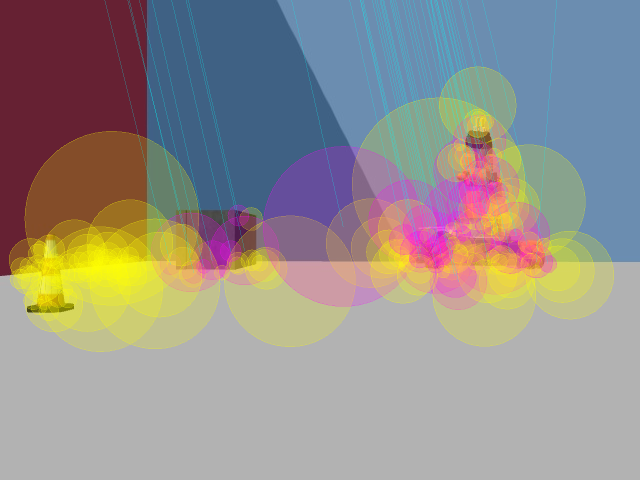
\includegraphics[height=5.5cm]{slam_house_features_corner_1}
\caption{text}
\end{minipage}
\hspace{1cm}
\begin{minipage}{0.45\textwidth}
\centering
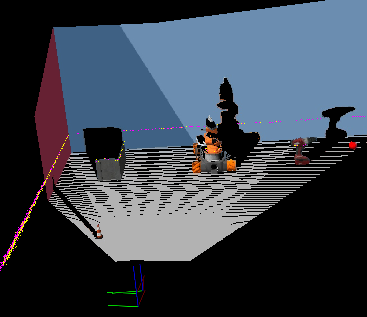
\includegraphics[height=5.5cm]{slam_house_constraints_1}
\caption{text}
\end{minipage}
\end{figure}

\begin{figure}[h]
\centering
\begin{minipage}{0.45\textwidth}
\centering
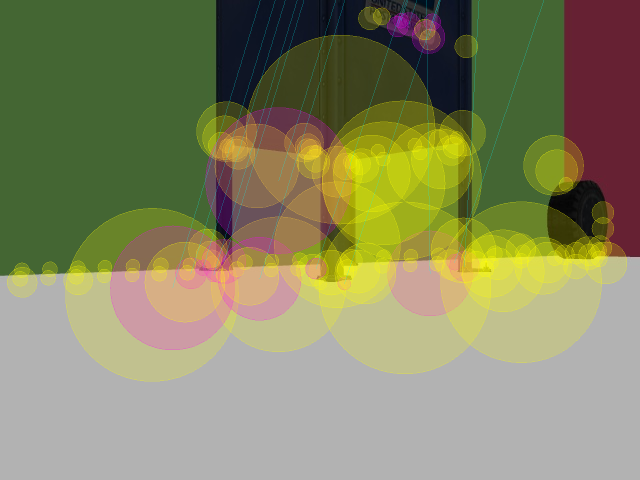
\includegraphics[height=5.5cm]{slam_house_features_corner_2}
\caption{text}
\end{minipage}
\hspace{1cm}
\begin{minipage}{0.45\textwidth}
\centering
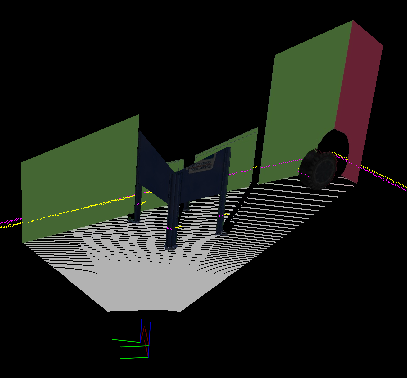
\includegraphics[height=5.5cm]{slam_house_constraints_2}
\caption{text}
\end{minipage}
\end{figure}

\begin{figure}[h]
\centering
\begin{minipage}{0.45\textwidth}
\centering

\includegraphics[height=5.5cm]{slam_house_features_corner_3}
\caption{text}
\end{minipage}
\hspace{1cm}
\begin{minipage}{0.45\textwidth}
\centering
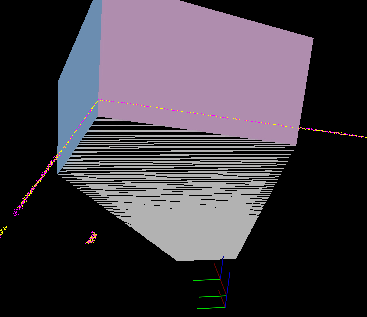
\includegraphics[height=5.5cm]{slam_house_constraints_3}
\caption{text}
\end{minipage}
\end{figure}

\begin{figure}
\centering
\frame{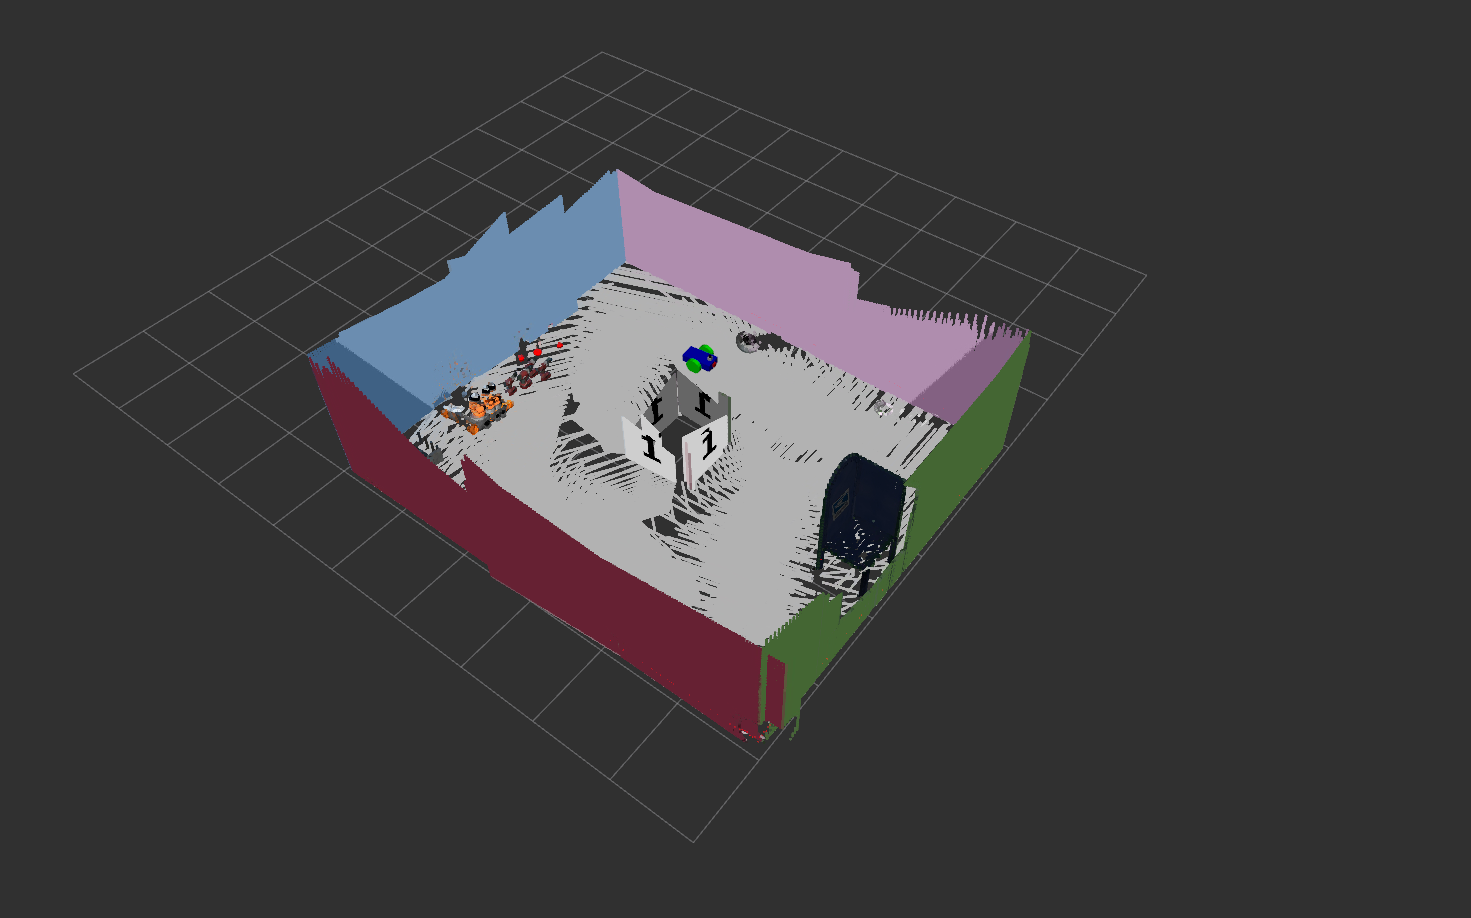
\includegraphics[scale=0.35]{slam_house_2_3d_map}}
\caption{text}
\end{figure}

\section{Discussion}
Discussion - The student explains how the procedure went and methodologies to improve it. The student should compare and contrast the performance of RTAB Mapping in different worlds.


\section{Future Work}


\bibliography{my_bib}
\bibliographystyle{ieeetr}

\end{document}